\section{Auswertung}
\label{sec:Auswertung}
\subsection{Bestimmung der Wagengeschwindigkeit}
Zunächst wird die Wagengeschwindigkeit bei den zehn verschiedenen Gangeinstellungen des Wagens, wie in Kapitel \ref{sec:d1} beschrieben, bestimmt.
Die Weglänge wird mithilfe eines Maßbandes zu
\begin{align*}
  s = \SI{43.8 +- 0.1}{\centi\metre}
\end{align*}
bestimmt.
Der jeweilige nominelle Wert für $t$ wird aus dem Mittelwert der fünf Einzelmessungen bestimmt.
Der Mittelwert berechnet sich dabei mithilfe der Formel
\begin{equation}
 \bar{x} = \frac{1}{n} \sum_{i=1}^n x_i.
\end{equation}
Der Fehler der Zeit wird mittels der Standardabweichung aus den fünf Einzelwerten bestimmt.
Die Standardabweichung berechnet sich dabei nach
\begin{equation}
  s = \sqrt{\frac{1}{n+1} \sum_{i=1}^n (x_i - \bar{x}) }.
\end{equation}
Unter der Annahme einer linearen Bewegung wird die Geschwindigkeit nun mit dem Weg-Zeit-Gesetz berechnet.
Für die Fehlerrechnung wird bei der vorliegenden Rechnung und bei allen folgenden Rechnungen das Gaußsche Fehlerfortpflanzungsgesetz
\begin{equation}
\increment{f} = \sqrt{\Bigl(\frac{\partial f}{\partial x_1}\increment{x_1}\Bigr)^2 + \Bigl(\frac{\partial f}{\partial x_2}\increment{x_2}\Bigr)^2 + \dotsc + \Bigl(\frac{\partial f}{\partial x_n}\increment{x_n}\Bigr)^2}
\end{equation}
für eine Funktion $f(x_1,x_2, \dotsc ,x_n)$, bei der die Größen $x_1, x_2, \dotsc , x_n$ voneinander unabhängig sind, verwendet.
Es ergeben sich hieraus die in Tabelle \ref{tab:Geschwindigkeiten} angegebenen Werte.\\

\begin{table}[H]
  \centering
  \caption{Wagengeschwindigkeiten}
  \label{tab:Geschwindigkeiten}
  \sisetup{table-format=1.2}
  \begin{tabular}{c c c}
    \toprule
    {$\text{Gang}$} & {$v [\si{\centi\metre\per\second}]$} & {$\increment v [\si{\centi\metre\per\second}]$}\\
    \midrule
    \input{build/geschwtabelle.tex}
    \bottomrule
  \end{tabular}
\end{table}

\subsection{Bestimmung der Ruhefrequenz}
Als nächstes wird die Ruhefrequenz $\nu_0$, wie in der Durchführung in Kapitel \ref{sec:durch_fre} beschrieben, bestimmt.
Dazu werden in einem Zeitintervall von $t = \SI{10}{\second}$ die im Empfänger aufgenommenen Schwingungen gemessen.
Es werden 7 Messungen durchgeführt, dessen Mittelwert und Standardabweichung sich zu
\begin{align*}
  \nu_0 &= \input{build/f_0.tex}
\end{align*}
ergeben und somit der Ruhefrequenz entsprechen.


\subsection{Bestimmung der Schallgeschwindigkeit}
Die Schallgeschwindigkeit wird, wie in Kapitel \label{sec:schall} beschrieben, mittels eines Präzisionsschlitten bestimmt.
Es werden dabei jeweils die Werte zwischen zwei benachbarten Extrema gleicher Phase verglichen.
Der sich aus Mittelwert sowie Standardabweichung ergebene Wert für $\lambda_0$, der Wellenlänge der Ruhefrequenz, ergibt sich zu
\begin{align*}
  \lambda_0 &= \input{build/wl.tex}
\end{align*}
sowie der Kehrwert der Wellenlänge zu
\begin{align*}
  \frac{1}{\lambda_0} &= \input{build/einsdurchwl.tex}
\end{align*}

Aus der Formel \ref{eqn:4.5} sowie dem zuvor bestimmten Wert der Ruhefrequenz ergibt sich eine Schallgeschwindigkeit von
\begin{align*}
  c &= \input{build/c.tex},
\end{align*}

\subsection{Bestimmung der Frequenzdifferenzen}
\label{sec:aa1}
Im Folgenden wird der Wagen in Bewegung gesetzt und die Frequenzdifferenzen, wie in Kapitel \ref{sec:durch_fre} beschrieben, bestimmt.
Für die zehn zuvor bestimmten Geschwindigkeiten werden die Anzahl der am Empfänger erreichten Schwingungen notiert.
Der betrachtete Zeitraum beträgt wiederum $t = \SI{10}{\second}$.
Aus den 5 Einzelmessungen wird jeweils ein Mittelwert sowie eine Standardabweichung gebildet.
Dementsprechend ergeben sich die in Tabelle \ref{tab:diffe} angegebenen Differenzfrequenzen $\nu_{\text{diff}}$ zu den jeweiligen Geschwindigkeiten $v$, wobei die gemessenen Frequenzen im Vergleich zu den zuvor bestimmten Ruhefrequenzen betrachtet werden.
\begin{table}
  \centering
  \caption{Frequenzdifferenzen durch Doppler-Effekt.}
  \label{tab:diffe}
  \sisetup{table-format=1.2}
  \begin{tabular}{c c c c}
    \toprule
    {$v [\si{\centi\metre\per\second}]$} & {$\increment{v} [\si{\centi\metre\per\second}]$} & {$\nu_{\text{diff}} [\si{\hertz}]$} & {$\increment{\nu_{\text{diff}}} [\si{\hertz}]$}\\
    \midrule
    \input{build/divtabelle_1.tex}
    \bottomrule
  \end{tabular}
\end{table}
Obwohl theoretisch 10 Geschwindigkeiten möglich sind, können bei der Vorwärtsbewegung jeweils nur die ersten sieben sowie bei der Rückwärtsbewegung nur die ersten sechs Geschwindigkeiten betrachtet werden.
Grund dafür ist, dass der Empfänger bei zu großer Distanz zum Lautsprecher keine zuverlässigen Werte mehr liefern kann.\\

Die berechneten Frequenzen können gegen die Geschwindigkeit aufgetragen werden.
Es ergibt sich ein linearer Zusammenhang, welcher linear an die Funktion
\begin{align*}
  y = m x + b
\end{align*}
gefittet wird.
Der Fit wird dabei in Python mit SciPy erstellt.
Es ergeben sich für die Ausgleichsgerade die Parameter
\begin{align*}
  c &= \input{build/propfak_1.tex}, \\
  b &= \input{build/bwert1.tex}.
\end{align*}
Der Parameter entspricht $c$ dabei laut Formel \ref{eqn:5} näherungsweise $\frac{ \nu_0}{c}$.
Der sich ergebende Plot ist in Abbildung \ref{afig:1} dargestellt.
\begin{figure}
  \centering
  \includegraphics{1plot.pdf}
  \caption{Frequenzdifferenz in Abhängigkeit der Relativgeschwindigkeit.}
  \label{afig:1}
\end{figure}

\subsection{Bestimmung der Frequenzdifferenzen mittels Schwebungsmethode}
Zudem können die Frequenzdifferenzen mithilfe der in Kapitel \ref{sec:d3} beschriebenen Schwebungsmethode erfasst werden.
Es können für die ersten fünf Geschwindigkeiten jeweils drei Messwerte aufgenommen werden, es wird nur die Rückwärtsbewegung der Reflexionsplatte betrachtet.
Aus den drei Werten wird wiederum ein Mittelwert und eine Standardabweichung gebildet.
Die Ergebnisse für die Frequenzdifferenz $\nu_{\text{diff}}$ wird mit den dazugehörigen Geschwindigkeiten in Tabelle \ref{tab:diffe2} dargestellt.
\begin{table}
  \centering
  \caption{Frequenzdifferenzen durch Doppler-Effekt mithilfe der Schwebungsmethode.}
  \label{tab:diffe2}
  \sisetup{table-format=1.2}
  \begin{tabular}{c c c c}
    \toprule
    {$v [\si{\centi\metre\per\second}]$} & {$\increment{v} [\si{\centi\metre\per\second}]$} & {$\nu_{\text{diff}} [\si{\hertz}]$} & {$\increment{\nu_{\text{diff}}} [\si{\hertz}]$}\\
    \midrule
    \input{build/divtabelle_2.tex}
    \bottomrule
  \end{tabular}
\end{table}
Es ergeben sich Werte, für die eine lineare Ausgleichsrechnung analog zur vorherigen Rechnung durchgeführt wird.
Hierbei ergeben sich die Fitparameter zu
\begin{align*}
  c &= \input{build/propfak_2.tex}, \\
  b &= \input{build/bwert2.tex}.
\end{align*}
Der Parameter $c$ entspricht wiederum laut Formel \ref{eqn:5} näherungsweise $\frac{ \nu_0}{c}$.
Die dargestellten Werte mit Ausgleichsgerade sind in Abbildung \ref{afig:2} dargestellt.
\begin{figure}
  \centering
  \includegraphics{2plot.pdf}
  \caption{Frequenzdifferenz in Abhängigkeit der Relativgeschwindigkeit aus Schwebungsmethode.}
  \label{afig:2}
\end{figure}
%\begin{figure}
%  \centering
%  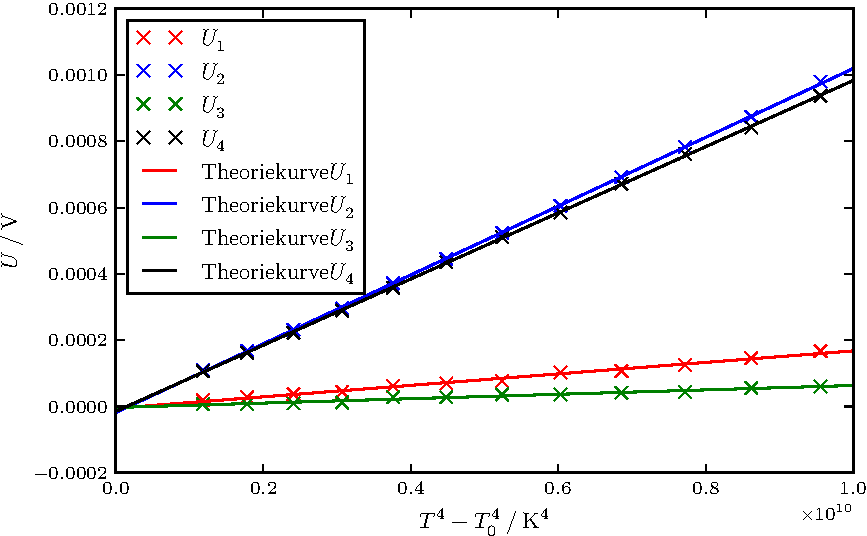
\includegraphics{plot.pdf}
%  \caption{Plot.}
%  \label{fig:plot}
%\end{figure}
%
%\begin{table}
%  \centering
%  \caption{Beispieltabelle}
%  \label{tab:tabelle_beispiel}
%  \sisetup{table-format=1.2}
%  \begin{tabular}{c c}
%    \toprule
%    {$a [\si{\second}]$} & {$b [\si{\kelvin}]$}\\
%    \midrule
%    1.0000  & 11.00 \\
2.0000  & 12.00 \\
3.0000  & 13.00 \\
4.0000  & 14.00 \\
5.0000  & 15.00 \\
6.0000  & 16.00 \\
7.0000  & 17.00 \\
8.0000  & 18.00 \\
9.0000  & 19.00 \\
10.0000 & 20.00 \\

%    \bottomrule
%  \end{tabular}
%\end{table}
%
%Es ergibt sich
%\begin{align}
%  a &= (0 \pm 0) ~ \si{\joule\per\kelvin\per\gram}
 \\
%\end{align}
